\documentclass[../INDE315_HW.tex]{subfiles} 
\usepackage{fancyhdr}
\usepackage{graphicx}
\usepackage{amsmath}
\usepackage{mhchem}
\usepackage{amssymb}
\usepackage[margin=1in]{geometry}

\graphicspath{{./images/}}

\title{UW IND E 315 Quiz 1}
\author{Anthony Le}

\begin{document}

\pagestyle{fancy}
\fancyhead{}
\fancyhead[R]{UW IND E 315}
\fancyhead[L]{Anthony Le}

\fancyhead[C]{Quiz 1}

\begin{center}
    \LARGE{\textbf{IND E 315 Quiz 1}}
\end{center}

\section*{Question 1}
Consider the following scenario: \\
Samples of emissions from three suppliers are classified for conformance to air-quality specifications. The results from 100 samples are summarized as follows:
\begin{center}
    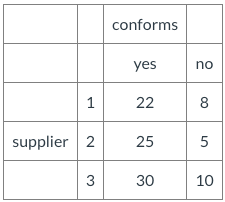
\includegraphics[width = 5cm]{Quiz1_Question1}
\end{center}
Let A denote the event that a sample is from supplier 1, and let B denote the event that a sample from any supplier conforms to specifications. If a disk is selected at random, determine the following probabilities. \\
Input your answers in the fractional form (do not simplify).

\subsection*{Question 1 Work}
\begin{enumerate}
    \item Finding $P(A)$
        \begin{enumerate}
            \item Sum up all samples from supplier 1, regardless of conformity, and divide by total number of samples.
        \end{enumerate}
        \begin{equation*}
            \begin{aligned}
                P(A) &= \frac{22+8}{100} \\
                     &= 30/100
            \end{aligned}
        \end{equation*}
    \item Finding $P(B')$
        \begin{enumerate}
            \item Sum up all samples that do not conform to specifications, regardless of supplier, and divide by total number of samples.
        \end{enumerate}
        \begin{equation*}
            \begin{aligned}
                P(B') &= \frac{8 + 5 + 10}{100} \\
                     &= 23/100
            \end{aligned}
        \end{equation*}
    \item Finding $P(A \cap B)$
        \begin{enumerate}
            \item Find the intersection for samples from supplier 1 AND meet specifications, and divide by total number of samples.
        \end{enumerate}
        \begin{equation*}
            \begin{aligned}
                P(A \cap B) &= \frac{22}{100} \\
                     &= 22/100
            \end{aligned}
        \end{equation*}
    \item Finding $P(A \cup B)$
        \begin{enumerate}
            \item Sum up all supplies that are from supplier 1, OR that meet specifications. Then divide by total number of samples.
        \end{enumerate}
        \begin{equation*}
            \begin{aligned}
                P(A \cup B) &= \frac{22 + 8 + 25 + 30}{100} \\
                        &= 85/100
            \end{aligned}
        \end{equation*}
    \item Finding $P(A' \cup B)$
        \begin{enumerate}
            \item Sum up all supplies that are NOT from supplier 1, OR that meet specifications. Then divide by total number of samples.
        \end{enumerate}
        \begin{equation*}
            \begin{aligned}
                P(A' \cup B) &= \frac{25 + 30 + 8 + 5 + 10}{100} \\
                        &= 78/100
            \end{aligned}
        \end{equation*}
\end{enumerate}

\section*{Question 2}
The following table summarizes the number of deceased beetles under autolysis (the destruction of a cell after its death by the action of its own enzymes) and putrefaction (decomposition of organic matter, especially protein, by microorganisms, resulting in production of foul-smelling matter):
\begin{center}
    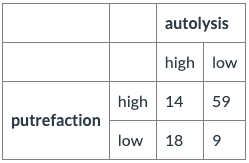
\includegraphics[width = 5cm]{Quiz1_Question2}
\end{center}
Let A denote the event that autolysis is high and let B denote the event that putrefaction is high. The total number of experiments is 100.

\subsection*{Question 2 Work}
\begin{enumerate}
    \item If the autolysis of a sample is high, what is the probability that the putrefaction is low?
        \begin{equation*}
            \begin{aligned}
                P(A \cap B') = 18/100
            \end{aligned}
        \end{equation*}
    \item If the putrefaction of a sample is high, what is the probability that the autolysis is high?
        \begin{equation*}
            \begin{aligned}
                P(A \cap B) = 14/100
            \end{aligned}
        \end{equation*}
    \item If the putrefaction of a sample is low, what is the probability that the autolysis is low? 
        \begin{equation*}
            \begin{aligned}
                P(A' \cap B') = 9/100
            \end{aligned}
        \end{equation*}
\end{enumerate}

\section*{Question 3}
The probability is 1\% that an electrical connector that is kept dry fails during the warranty period of a portable computer. If the connector is ever wet, the probability of a failure during the warranty period is 5\%. If 90\% of the connectors are kept dry and 10\% are wet, what proportion of connectors fail during the warranty period?

\subsection*{Question 3 Work}
\begin{enumerate}
    \item Assuming that wet and dry connectors are independent from each other, having no impact on each other.
    \item Assuming that A represents the failure of dry connectors, and B represents the failure of wet connectors
    \begin{equation*}
        \begin{aligned}
            P(A) &= 1\% * 90\% \\
                &= 0.9\% \\
            P(B) &= 5\% * 10\% \\
                &= 0.5\% \\
            P(A \cup B) &= P(A) + P(B) \\
                &= 0.9\% + 0.5\% \\
                &= 1.4\% \quad \text{or} \quad 0.0140
        \end{aligned}
    \end{equation*}
\end{enumerate}

\section*{Question 4}
Consider the well failure data given below. Let A denote the event that the geological formation of a well has more than 1000 wells, and let B denote the event that a well failed.
\begin{center}
    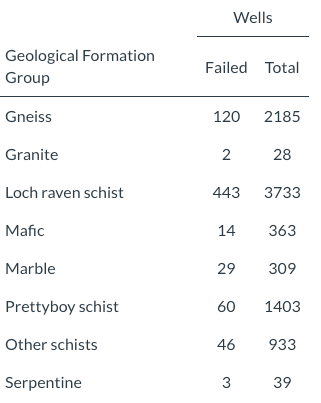
\includegraphics[width = 5cm]{Quiz1_Question4}
\end{center}
Are A and B independent?

\subsection*{Question 4 Work}
Yes, they are independent from each other. However, this comes with the assumption that the well failure has no impact on the total well count - since we're not given information about how the total well count is determined.



\end{document}